\begin{figure}
    \centering
    \begin{subfigure}[b]{0.49\textwidth}
        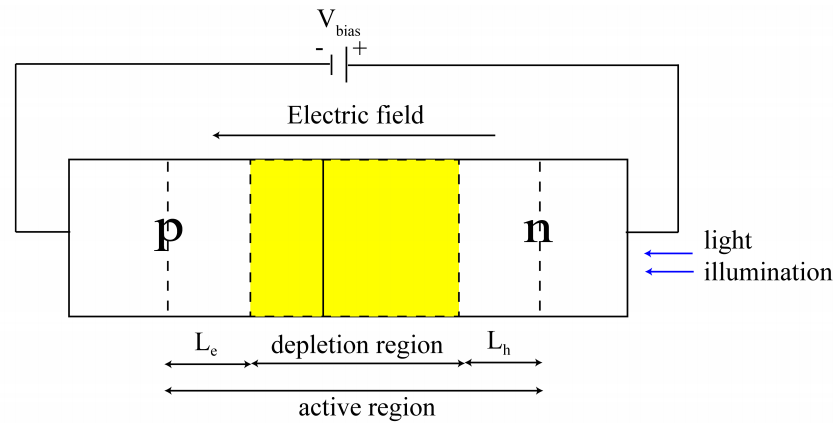
\includegraphics[width=\linewidth,keepaspectratio]{figures/background/cmos/photodiode.png}
        \caption{Photodiode schematic. L\textsubscript{e}, L\textsubscript{h} are electron, hole diffusion lengths respectively\cite{Xu2015FundamentalCO}.}
        \label{fig:photodiode.png}
    \end{subfigure}
    \vskip\baselineskip
    \begin{subfigure}[b]{0.49\textwidth}
        \center
        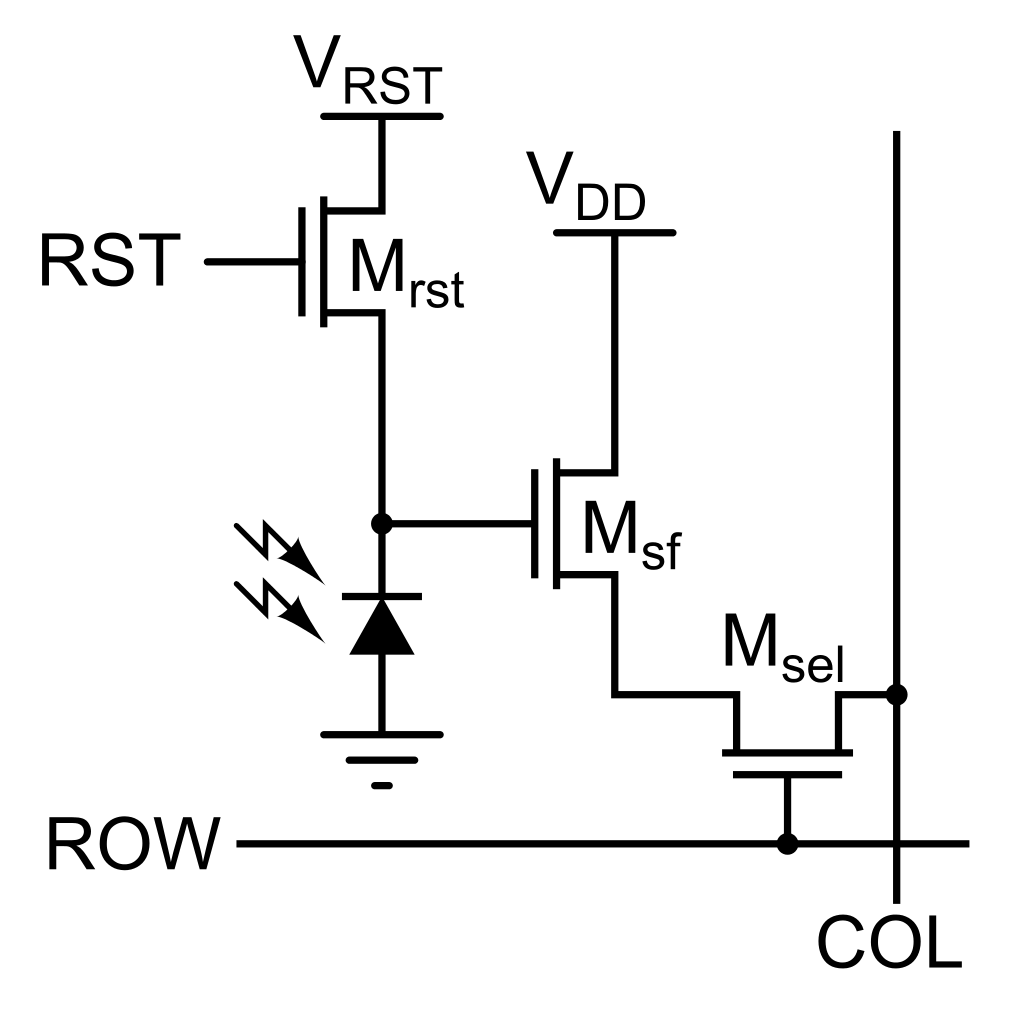
\includegraphics[width=.8\linewidth,keepaspectratio]{figures/background/cmos/3t_pixel.png}
        \caption{Three transistor pixel. M\textsubscript{rst} is the reset transistor (enabling the photodiode to dump charge), M\textsubscript{sf} buffers the charge on the photodiode (so that it can be read without loss), and M\textsubscript{sel} enables a whole row of pixels to be read simultaneously (since all pixels in a physical row are tied to the same row line).}
        \label{fig:3tpixel}
    \end{subfigure}
    \caption{CMOS components.}
\end{figure}